\chapter{Statistical analysis}\label{chap:stats}

The interpretation of measured observables after performing a measurement forms one of the main challenges in experimental particle physics. Statistical methods are used to quantify the relationship between some measured observables and parameters in a model. In the analysis described in this thesis, the goal is estimating the number of non-resonant signal events from the measured dataset, containing possibly both signal and background events. The estimated signal yield and the estimated background yield can be used to determine the agreement of non-resonant, i.e. Contact Interactions scenarios with data, and infer values of parameters in non-resonant models. 

A central concept in statistics in particle physics is that of uncertainty, which can originate from several different sources. For example, uncertainties can be the result of the lack of knowledge of the experiment, or the consequence of a more fundamental random nature in the system due to quantum mechanics. A variable is said to be random when it is not known or cannot be predicted with complete certainty~\cite{Cowan1998}. The concept of probability can be used to quantify the degree of randomness. Kolmogorov formulated a mathematical definition of probability as a set of axioms~\cite{Kol33}. 

The interpretation of probability can take two forms. The frequentist interpretation, and another known as subjective or Bayesian probability is also used. The frequentist notion of probability of an event is defined as the limit of its relative frequency in a large number of trials. A large number of trials forms an ensemble, where in particle physics an ensemble can be formed by repeating the experiment multiple times. In frequentist probabilities, the true values of the parameters are states of nature and not the outcome of the experiment. The Bayesian definition of probability is based on a degree of belief. Therefore, Bayesian probabilities can be assigned to hypothesis on states of nature. The practical consequence of Bayesian probabilities is that prior must be supplied for various parameter values and hypothesis. 

The frequentist interpretation of probability is used for analysis in this thesis. The prevalent use of the frequentist interpretation does not indicate an inherent merit over the Bayesian interpretation, but rather highlights the technically simple implementation of the frequentist interpretation. 

\section{Parameter estimation}
One of the most common tasks in high energy physics is an estimation of some model parameter, commonly known as the parameter of interest (POI), e.g. a number of signal events or signal strength in search for new physics. The POI can be estimated by measuring a set of \emph{observables}, \emph{x}, whose probability depends on the POI. Depending on the analysis, different quantities can be utilised as \emph{observables}, e.g. the analysis described in this thesis uses the dielectron and dimuon invariant mass. Replication of the experiment multiple times results in different values of \emph{x}, which results in a \emph{probability density function} of \emph{x}, written as $f(x;\alpha)$. The probability density function has the important property of satisfying the normalisation condition
\begin{equation}
    \begin{aligned}
        \int_{-\infty}^{\infty} f(x;\alpha)~dx = 1,
    \end{aligned}
\end{equation}

where the parameter $\alpha$ represents some unknown parameter. $f(x)$ describes the probability density for a single event. However, when considering datasets with many events, $\mathcal{D} = (x_1,..,x_n)$, the probability density is given by the product of the densities for each event. In counting experiments, such as the one described in this analysis, the total number of selected events is also a random variable, where the total number of observed events, \emph{n}, fluctuates around the expected number of events, $\nu$, according to a Poisson distribution. When considering binned data, common to most analyses, histograms are defined that yield a certain number of entries $\textbf{n} = (n_1,..,n_N)$ in \emph{N} bins. The expected number of events in the entries for a bin is given by
\begin{equation}
\begin{aligned}
    \nu_i(\alpha) = n_{tot}\int_{x_i^{min}}^{x_i^{max}} f(x;\alpha)~dx,
\end{aligned}
\end{equation}
where $x_{min}$ and $x_{max}$ are the bin limits, and $n_{tot}$ is the total number of events in the dataset. A likelihood function for the total probability distribution for \emph{N} bins can be defined:
\begin{equation}
    \label{eq:poissL}
    \begin{aligned}
        & \mathcal{L}(n;\alpha) = \prod_{i=1}^{N}\frac{\nu_{i}^{n_{i}} e^{-\nu_{i}}}{n_{i}!}. \\
    \end{aligned}
\end{equation}

For the single-bin counting experiment used in the analysis $N = 1$ due to only one bin used for the statistical analysis. The expected number of events in the bin can be defined as $\nu = \nu_B +\nu_S$, where $\nu_B$ is the expected background events, and $\nu_S$ is the expected signal events in the bin. The POI used in this analysis is $\nu_S$. Using the likelihood function, one can estimate the POI given the collected data. 

An \emph{estimator}, $\hat{\alpha}(\mathcal{D})$ is some function of the data and its value is used to estimate the true value of some parameter $\alpha$. There are various properties that an estimator must satisfy to be considered a \emph{good} estimator, e.g. bias, variance, consistency~\cite{errorsOnNumbers}. Consistency is the requirement that the estimator should converge to the true value in the limit of infinite statistics. A bias of an estimator is defined as the difference between the expectation value of the estimator, $E[\hat{\alpha}]$, and the true value of $\alpha$. Variance is defined as $var[\hat{\alpha}] = E\left[(\alpha - E[\hat{\alpha}])^{2}\right]$. There is a clear trade-off between bias and variance, in the class of unbiased estimators, there is a well-defined minimum variance bound~\cite{Cranmer:2015nia}. When interpreting the results in the context of CI interaction models, $\nu_S$ can be expressed as a function of $\Lambda$, where $\Lambda$ can also be considered the POI. This allows for the results to be either interpreted directly in terms of lambda or the reinterpretation of the results from  the number of signal events, $\nu_s$.

The most commonly used estimator is the maximum likelihood estimator (MLE), defined as the value of $\alpha$, which maximises the likelihood function. In practice, due to computational efficiency, this is done by minimising $-\log\mathcal{L}$. For multi-parameter likelihood functions, the various components of $\alpha_p$ are referred to as \emph{floating} parameters. The MLE method can be generalised and is used in determining determine the \emph{best-fit} values for the parameters used in the background estimation. The minimisation is handled by the Minuit~\cite{James:873119} tool in the RooFit framework.

\subsubsection{Combination of channels}
Probability models can be constructed to describe several channels defined by some associated selection criteria simultaneously. The likelihood in \cref{eq:poissL} can be redefined for the combination of electron and muon channels,
\begin{equation}
    \label{eq:poissLcomb}
    \begin{aligned}
        & \mathcal{L}(n;\alpha) = \prod_{\mathrm{c}~\in~\mathrm{channels}}~\frac{\nu_{c}^{n_{c}} e^{-\nu_{c}}}{n_{c}!}, \\
    \end{aligned}
\end{equation}
where the models for the individual channels are multiplied together. For simplicity of notation, the discussion below focuses only on a single channel. However, the procedure described below is applied to the combined model as well. 

\section{Treatment of systematic uncertainties}\label{sec:stats:nps}
In the example likelihood given in \cref{eq:poissL}, there are additional parameters that also affect the distributions of the observables that are not the POI. These parameters are known as \emph{nuisance parameters} ($\theta$), since they must be accounted for regardless of the interest to the analysis. These include the systematic uncertainties affecting the signal and background normalisation and shape. Using the methods described in \cref{sec:extrap:uncertainties}, $\pm 1\sigma$ up and down variations of $\tilde{\theta}$ are constructed. Once the uncertainties have been estimated, a constraint term $f(\tilde{\theta};\theta,\sigma_\theta)$ is multiplied by the likelihood. A Gaussian penalty term is used for the constraint term in the analysis. The Gaussian constraint is parameterised such that $\tilde{\theta} = 0$ is the nominal value of the parameter, and $\tilde{\theta} \pm 1$ are the $\pm1\sigma$ variations. The likelihood can be redefined as:
\begin{equation}
    \label{eq:likelihood}
    \begin{aligned}
        & \mathcal{L}(n;\nu,\theta) = \frac{\nu(\nu_s,\theta)^{n} e^{-\nu(\nu_s,\theta)}}{n!} \times \prod_{j=1}^{N_{syst}} \frac{1}{\sqrt{2\pi}\sigma_{\theta,j}} e^\frac{-(\tilde{\theta_j} - \theta_j)}{2\sigma_{\theta,j}^2} \\
    \end{aligned}
\end{equation}
where $\theta_j$ is the nuisance parameter corresponding to systematic \emph{j}. 

When the data is fit using the full likelihood in \cref{eq:likelihood}, both the POI and nuisance parameters are estimated to minimise the likelihood. However, in some scenarios, the fit may constrain a nuisance parameter better than the POI, indicating an inherent mismodelling of the likelihood. Over constraining nuisance parameters may lead to underestimated uncertainties on the POI. The \emph{post-fit} pulls are used to quantify the degree to which the estimate of the nuisance parameter, $\hat{\theta}$, deviates from the expected value, $\tilde{\theta}$, given the uncertainty after fitting, $\hat{\sigma}$. The pull of a nuisance parameter is defined as
\begin{equation}
    \label{eq:nppull}
    \begin{aligned}
        & \mathrm{pull} = \frac{\hat{\theta} -{\theta}}{\hat{\sigma_\theta}}.
    \end{aligned}
\end{equation}
Deviation from the central value of the nuisance parameter will indicate features of the data not described by the model. The pulls of the nuisance parameters from the fit to data are shown in \cref{chap:results}. The impact of the nuisance parameter on the parameter of interest is defined as:
\begin{equation}
    \label{eq:npinpact}
    \begin{aligned}
        & \mathrm{Impact} = \Delta \hat{\nu_s} = \hat{\hat{\nu}}_{s,\theta \pm \sigma_\theta} - \hat{\nu}_s,
    \end{aligned}
\end{equation}
where, $\hat{\hat{\nu}}_{s,\theta \pm \sigma_\theta}$, is the fitted value of $\nu_s$ with the nuisance parameter fixed at at it's expectation value plus or minus it's standard deviation, resulting in the \emph{prefit} impact. The postfit impact given by the nuisance parameter fixed at its observed value plus or minus its standard deviation. 


\section{Hypothesis tests}
Hypothesis tests are an additional statistical tool used in the analysis to test the compatibility of the data collected with respect to two hypotheses, rejecting one over the other based on experimental observations. Two hypotheses are defined: an \emph{alternative hypothesis} ($\mathrm{H_0}$) and a \emph{null hypothesis} ($\mathrm{H_0}$). When considering an observed excess for discovery, $\mathrm{H_0}$ is defined as the expectation solely based on the SM background expectation, also referred to as the background-only hypothesis. While $\mathrm{H_1}$ is defined as the expectation from SM background and a BSM process, e.g. CIs, is referred to as the signal+background hypothesis. The claim of discovery is that the data are incompatible with the background-only hypothesis. When no significant excess is observed, the incompatibility of the data with signal+background hypothesis is tested, and a potential signal can be excluded. 

In order to distinguish between the two hypothesis a \emph{test statistic}, $\mathcal{T}(\mathcal{D})$ is constructed such that the value of $\mathcal{T}$ will be different dependant on the hypothesis. An \emph{acceptance region} is defined, such that if $\mathcal{T}(\mathcal{D}) < k_\alpha$, then $H_0$ is accepted. The test statistic is defined such that it minimises the probability at which $H_0$ is rejected when it is true, known as a Type-I error. In contrast, a Type-II errors describes accepting $H_0$ when $H_1$ is true, denoted by $\beta$. A test statistic is chosen such that it maximises the power of a test, $1-\beta$. There are a multitude of test statistics that can be used. The most powerful test is given by the likelihood ratio $\mathcal{T}(\mathcal{D}) = \mathcal{L}(n;\nu_{s+b})/\mathcal{L}(n;\nu_{b})$ according to the Neyman-Pearson lemma~\cite{Cowan1998}. A generalisation of the likelihood ratio known as the \emph{profile likelihood ratio} is defined as
\begin{equation}
    \label{eq:profLL}
    \begin{aligned}
        \lambda(\nu_s) = \frac{\mathcal{L}(\nu_s;\hat{\hat{\theta}}(\nu_s))}{\mathcal{L}(\hat{\nu}_s,\hat{\theta})},
    \end{aligned}
\end{equation}
where the \emph{conditional maximum likelihood estimate}, $\hat{\hat{\theta(\nu_s)}}$,  is the value of $\theta$ that maximises the likelihood function with $\nu_s$ fixed. The profile likelihood test statistic is used in many of the LHC experiments, including ATLAS. The test statistic is used to define the final test statistic relevant to analyses
\begin{equation}
    \label{eq:teststat}
    \begin{aligned}
        q_{\nu_s} = -2\ln\lambda(\nu_s),
    \end{aligned}
\end{equation}

where it is used to quantify the compatibility of the observed data for a given hypothesis. The probability to have obtained data with a certain property assuming a hypothesis~\cite{Cranmer:2015nia} is given by the \emph{p}-value, 
\begin{equation}
    \label{eq:pvalue}
    \begin{aligned}
        p_{\nu_s} = \int_{q_{\nu_{s},obs}}^\infty f(q_{\nu_s};\nu_s,\theta)~dq_\mu,
    \end{aligned}
\end{equation}
where $f(q_\mu;\nu_s,\theta)$ is the probability density function of the test statistic under the hypothesis $\nu_s$, $q_{\mu,obs}$ is the test statistic of the observed data. As $p_{\nu_s}$ gets smaller, the confidence that the assumed hypothesis is true decreases. 

For discovery, the null hypothesis ($\nu_s = 0$) must be rejected. This compatibility is based on the following \emph{p}-value
\begin{equation}
    \label{eq:pvalue_bonly}
    \begin{aligned}
        p_{0} = \int_{q_{\mu,obs}}^\infty f(q_0;0,\hat{\hat{\theta}}(\nu_s =0))~dq_\mu.
    \end{aligned}
\end{equation}
Incompatibilities with the null hypothesis at the level of $p_0 = 1.3 \times 10^{-3}$ and $p_0 = 2.9 \times 10^{-3}$ are required in order to state that observation and discovery, respectively. It is customary to convert the \emph{p}-value into the sigma (quartile) of a unit Gaussian, defined as
\begin{equation}
    \label{eq:sigma}
    \begin{aligned}
    Z = \Phi^{-1}(1-p_0),
    \end{aligned}
\end{equation}
where $\Phi^{-1}$ is the inverse of a cumulative distribution for a unit Gaussian. The significances for the observation and discovery correspond to $3\sigma$ and $5\sigma$, respectively.

When no significant excess is observed in data, a limit on the number of signal events or CI $\Lambda$ scale is set. For limit setting the test statistic, $\tilde{q}_{\nu_s}$, is used to differentiate the hypothesis of the signal being produced at $\nu_s$ from the alternative hypothesis at $\nu_s^\prime < \nu_s$,
\begin{equation}
    \label{eq:limitTestStat}
    \begin{aligned}
    \tilde{q}_{\nu_s} = \begin{cases}
        -2\ln\frac{\mathcal{L}(\nu_s,\hat{\hat{\theta}}(\nu_s))}{\mathcal{L}(0,\hat{\hat{\theta}}(0))} & \mathrm{for }~\hat{\nu_s} < 0, \\
        -2\ln\frac{\mathcal{L}(\nu_s,\hat{\hat{\theta}}(\nu_s))}{\mathcal{L}(\hat{\nu}_s,\hat{\theta})} & \mathrm{for }~0 \leq \hat{\nu}_s \leq \nu_s, \\
        0          & \mathrm{for }~\hat{\nu}_s > \nu.
    \end{cases}
    \end{aligned}
\end{equation}
A \emph{p}-value can be defined for the hypothesis using the above test statistic and \cref{eq:pvalue}, 
\begin{equation}
    \label{eq:pvalue_sb}
    \begin{aligned}
        p_{\nu_s} = \int_{\tilde{q}_{\mu,obs}}^\infty f(\tilde{q}_{\nu_s};\nu_s,\hat{\hat{\theta}}(\nu_s))~d\tilde{q}_\mu.
    \end{aligned}
\end{equation}
It was previously defined if the test statistic is outside the acceptance region $\alpha$, the hypothesis is rejected. Using this definition, the region at $p_{\nu_s} \geq 1 - \alpha$ is referred to as the \emph{confidence level} (CL) that includes the true value of the POI with probability larger than $1-\alpha$. This definition of CL would then lead to the statement that the confidence interval covers the true value of the parameter with a CL larger than $1-\alpha$. The CL value of the upper limit is commonly chosen as 95\% for ATLAS and CMS results. Signal hypothesis will be tested until the point at which the signal hypothesis is found that is no longer excluded at the 95\% confidence interval. 

The expected limit and corresponding upper and lower bounds are calculated by sampling a distribution of the limits produced from many background-only MC toy experiments and taking the median value of the expected limit distribution, and its 95\% and 68\% quantiles. The median value is taken instead of the mean, as it is invariant to the choice of significance or \emph{p}-value. The distribution of the limit is given by $f(\nu_{s,lim};0,\hat{\hat{\theta}}(\nu_s = 0,obs))$, where the nuisance parameters have a profiled value based on the observed data. The upper and lower bounds correspond to the $1\sigma$ and $2\sigma$ uncertainty on the expected limit.

\cref{fig:toyDist} depicts the distribution of limits from toy MC experiments in the constructive and destructive SRs in the electron and muon channel. The results are based on 2000 toy experiments. The 68\% and 95\% quantiles of the distribution corresponding to the one and two sigma error bands, respectively, are indicated on the distributions by the yellow and green bands. Non-Gaussian behaviour observed in the distributions lead to an asymmetry in the expected limit uncertainty; this is especially prominent in the muon destructive signal regions. 

\begin{figure}[!htpb]
    \centering
    \begin{subfigure}[b]{0.49\textwidth}
        \centering
        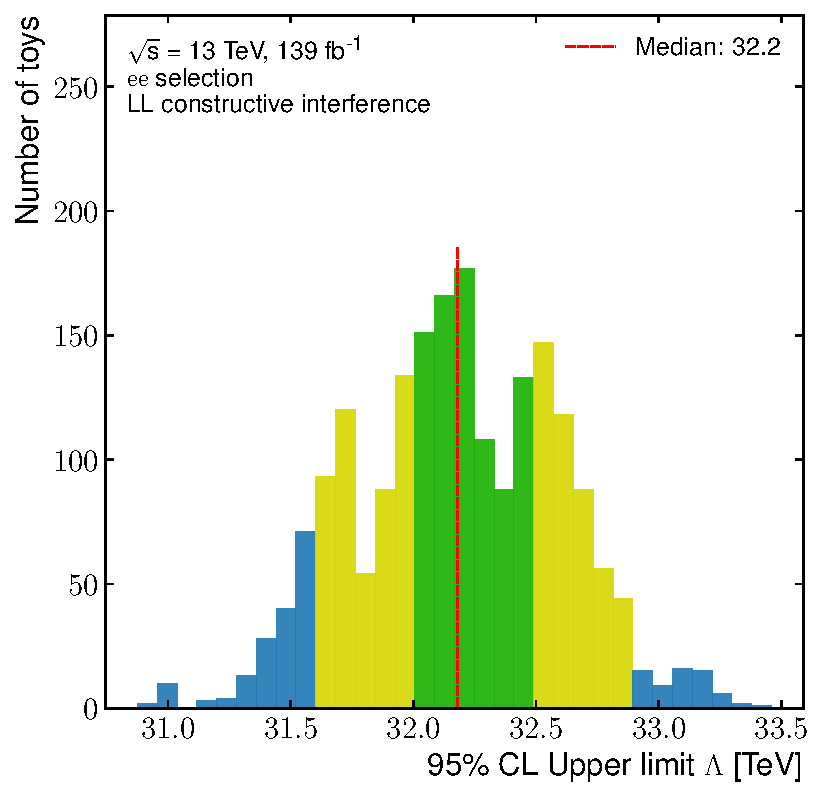
\includegraphics[width=\textwidth]{/Users/Deshan/Documents/PhD/thesis/Thesis/figures/analysis/stats/toyLimitDist-ee-const.pdf}
        \label{fig:toyDist1}
    \end{subfigure}
    \begin{subfigure}[b]{0.49\textwidth}
        \centering
        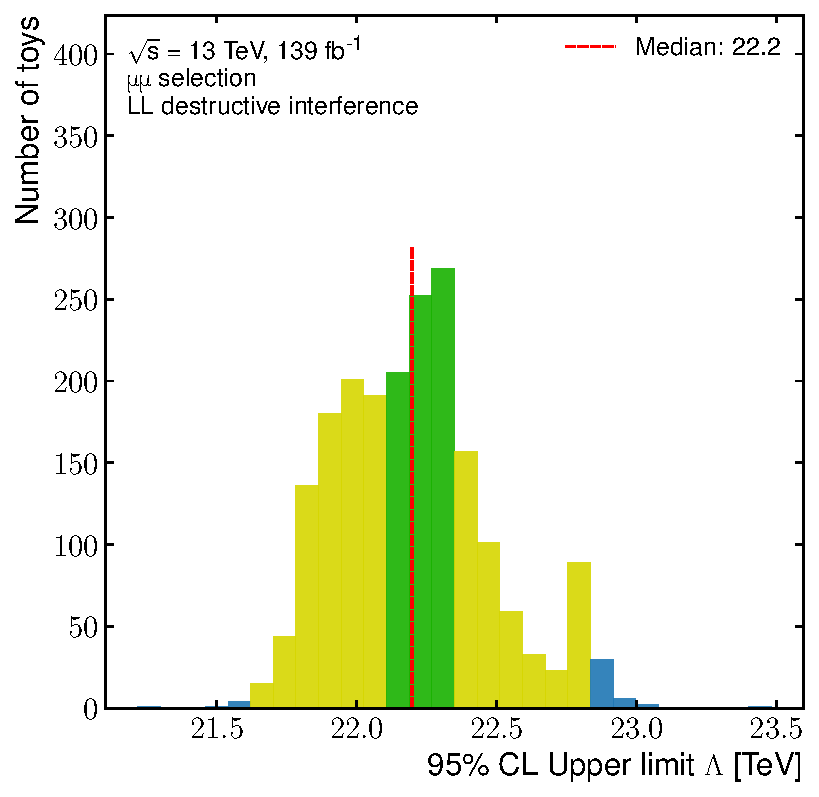
\includegraphics[width=\textwidth]{/Users/Deshan/Documents/PhD/thesis/Thesis/figures/analysis/stats/toyLimitDist-mm-dest.pdf}
        \label{fig:toyDist2}
    \end{subfigure}
    \caption[Expected limit distribution for 2000 toy MC experiments.]{Expected limit distribution for 2000 toy MC experiments in the electron constructive (left) and muon destructive (right) signal region for the LL CI model. The dashed line indicates the median of the distribution. The green and yellow bands correspond to the 68\% and 95\% quantiles, respectively, of the distribution.}
    \label{fig:toyDist}
\end{figure}

\subsubsection{$\mathrm{CL}_\mathrm{s}$ construction}
Once a statement on the exclusion of a model has been made, the model is no longer considered essential to be searched. Therefore, the metric by which analyses can claim a model has been excluded has been studied in great detail. The \emph{p}-value discussed above can be subjected to statistical fluctuations and can lead to non-physical exclusions when a downward fluctuation in the observed number of events occurs. This would result in premature exclusions of new physics models. 

Two methods are constructed to tackle this problem by the high energy physics community: the power-constrained limit (PCL)~\cite{PhysRevLett.122.231801} and the $\mathrm{CL}_\mathrm{s}$ formalism~\cite{JUNK1999435,Read_2002}. The PCL method is not used widely used in the community but represents a cutoff at a positive value of the POI everywhere. The more widely accepted, $\mathrm{CL}_\mathrm{s}$ formalism is constructed to reduce the likelihood of excluding signal hypotheses that a search is not otherwise sensitive. The $\mathrm{CL}_\mathrm{s}$ formalism is defined as the ratio of two \emph{p}-values:
\begin{equation}
    \label{eq:cls}
    \begin{aligned}
        \mathrm{CL}_\mathrm{s} = \frac{p_{\nu_{s+b}}}{1-p_{\nu_{b}}}
    \end{aligned}
\end{equation}
where $p_{\nu_{s+b}}$ and $p_{\nu_{b}}$ quantify the compatibility between the data and the signal+background and background-only hypothesis. The negative fluctuations will be moderated by the denominator, which is the same test statistic as the numerator, but with $\nu_s = 0$. $\mathrm{CL}_\mathrm{s}$ formalism is mainly used to perform hypothesis tests aimed at excluding signal models. 

\subsubsection{Asymptotic approximation}
In addition to the toy MC approach, the confidence interval can be calculated using asymptotic formulae~\cite{Cowan:2010js}. This approximation is based on theorems by Wilks and Wald~\cite{wilks1938}, which show that for sufficiently large data sample, the distribution of the likelihood-ratio based test statistic follows a Gaussian distribution. Therefore, $-2\ln\mathcal{L}(\nu_s)$ will follow a $\chi^2$ distribution. The probability $p_0$ can be directly calculated from $q_0$ as~\cite{Cowan:2010js}:
\begin{equation}
    \label{eq:p0_asymp}
    \begin{aligned}
        p_0 = 1 - \Phi\left(\sqrt{q_0}\right),
    \end{aligned}
\end{equation}
and the significance takes the form $Z = \sqrt{q_0}$. The asymptotic approach considerably reduces the computing time and resources required. 

Due to the assumed distribution of the test statistic, for Poisson-like distributions with low statistics, limits obtained using the asymptotic approximation may be optimistic. The single-bin signal regions defined at high invariant mass for the analysis has low statistic. Therefore, the asymptotic approximation is deemed insufficient for the analysis. A comparison of the expected limits from the toy MC method and the asymptotic approximation is shown in \cref{fig:asympVstoy}. The results from the asymptotic approach predict an expected limit that is optimistic compared to the toy approach. 

\begin{figure}[!htpb]
    \centering
    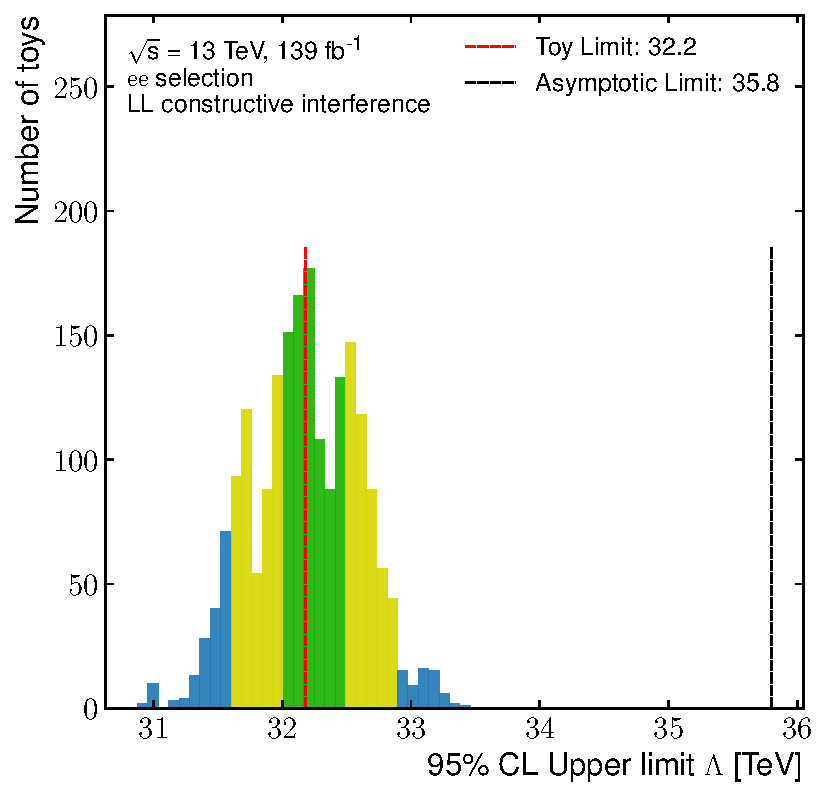
\includegraphics[width=0.7\textwidth]{/Users/Deshan/Documents/PhD/thesis/Thesis/figures/analysis/stats/toyLimitVsAsymp-ee-const.pdf}
    \label{fig:asympVstoy1}
    \caption[Comparison of expected limit from the toy MC method and the asymptotic approximation.]{Comparison of expected limit from the toy MC method and the asymptotic approximation in constructive electron signal region for the LL chiral CI model. The expected limit from the toy MC method and the asymptotic approximation is shown by the red and black dashed lines, respectively.}
    \label{fig:asympVstoy}
\end{figure}

\section{Choice of parameter of interest}\label{sec:stat:poi}
The formalism above focus on the number of signal events $\nu_s$ as the parameter of interest. This choice of POI allows to search for non-resonant signals and set limits in terms of the number of signal events in the signal region independent of any assumed signal models. There are two possible methods to interpret the results in terms of CI models: a reinterpretation of the model-independent limits in terms of CI models using the CI signal MC templates, and the other where the $\nu_s$ is parameterised in terms of the CI energy scale $\Lambda$ and limits are set on CI models directly.  

There are several steps involved with the reinterpretation of the model-independent limits in the context of CI models. The CI interaction signal MC is used to map the expected number of signal events for a given model to the number of signal events. The constructive signal region results are expected to be used for constructive interference CI models, whereas the destructive interference signal region results are used for destructive models. Once an interference model has been chosen, the limits on the number of signal events are mapped to the different chiral models of the CI reweighted templates described in \cref{sec:datamc:mc:sig}. A linear interpolation is performed between reweighted $\Lambda$ points to allow for signal events to be extracted between reweighted $\Lambda$ points. \cref{fig:stats:interpeeconst,fig:stats:interpeedest,fig:stats:interpmmconst,fig:stats:interpmmdest} depict the reinterpretation of the $\nu_s$ expected limits in the context of the CI $\Lambda$ limits. It is important to note that the uncertainty on the signal yield has not been taken into consideration. The procedure in including the uncertainties would involve taking the experimental uncertainty on the CI signal model and varying the expected yield by the uncertainty and calculating the corresponding limit. 

Interpretation of the results directly on the CI energy scale $\Lambda$ involves parametrising the expected signal yield, $\nu_s$ in terms of $\Lambda$. The parameterisation can be achieved by a small modification to the custom PDF class created described in \cref{sec:datamc:mc:sig:morphing}, where the integral of the expected number of signal events in the SR is provided as a function of $\Lambda$. This allows the POI to be defined as $\Lambda$. The expected number of events predicted in the signal yield can then be written as $\nu = \nu_b +\nu_s(\Lambda)$. An advantage of using $\Lambda$ as the POI is that it uses a common parameter between the electron and muon channels. This allows the likelihood to be defined for the combination of the electron and muon channels in terms of $\Lambda$. The limits set on the number of events for the combined channel has no trivial mapping to $\Lambda$. This is due to different signal yields can be predicted in the electron and muon channels for a given $\Lambda$ caused by the different detector efficiencies of electrons and muons. 

The expected limits in the electron and muon channels are compared for the two choices of POI in \cref{tab:limits_comparePOI}. The limits shown indicate that there is a little difference between interpreting the limits directly on $\Lambda$ and reinterpreting them from the limits on the number of signal events. Due to the added benefit of having limits on the combined electron and muon channels, the final results on the CI models are interpreted directly in terms of $\Lambda$. However, the model-independent limits on $\nu_s$ are still produced to facilitate reinterpretation into other non-resonant BSM models. 

\begin{figure}[h!]
    \centering
    \begin{subfigure}[b]{0.49\textwidth}
        \centering
        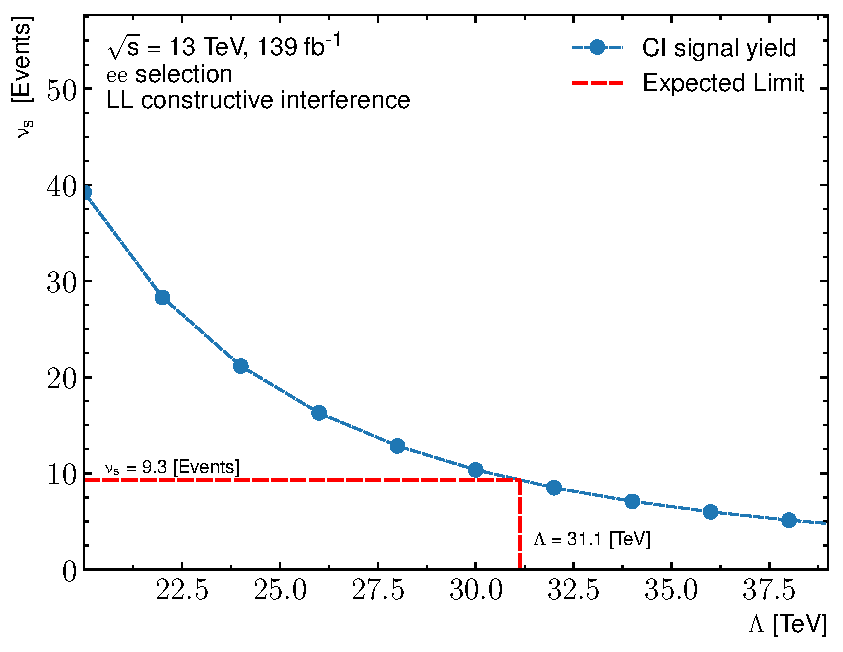
\includegraphics[width=\textwidth]{/Users/Deshan/Documents/PhD/thesis/Thesis/figures/analysis/stats/intersection-ee-const-LL.pdf}
        \label{fig:bkgmodel:interpee1}
    \end{subfigure}
    \begin{subfigure}[b]{0.49\textwidth}
        \centering
        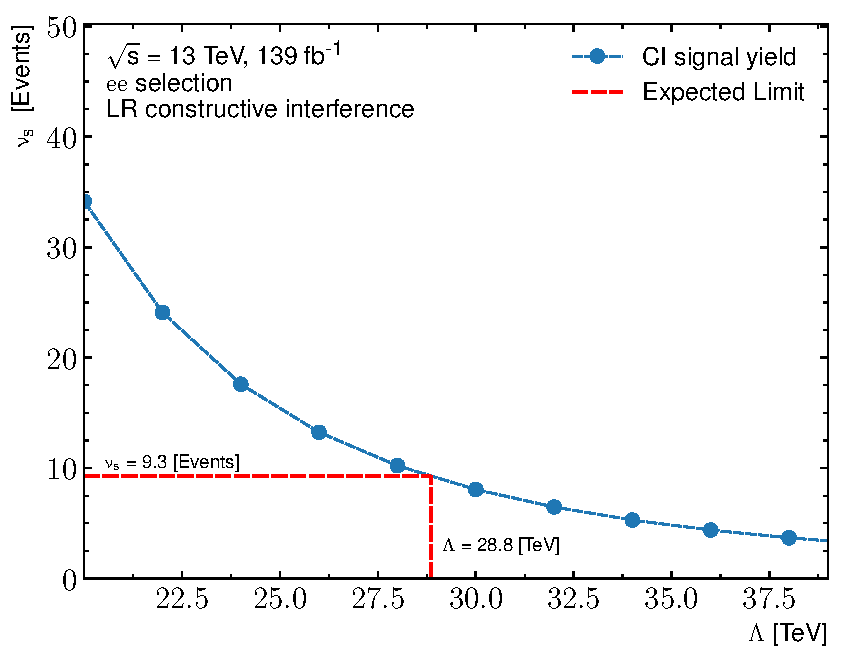
\includegraphics[width=\textwidth]{/Users/Deshan/Documents/PhD/thesis/Thesis/figures/analysis/stats/intersection-ee-const-LR.pdf}
        \label{fig:bkgmodel:interpee2}
    \end{subfigure}
    \begin{subfigure}[b]{0.49\textwidth}
        \centering
        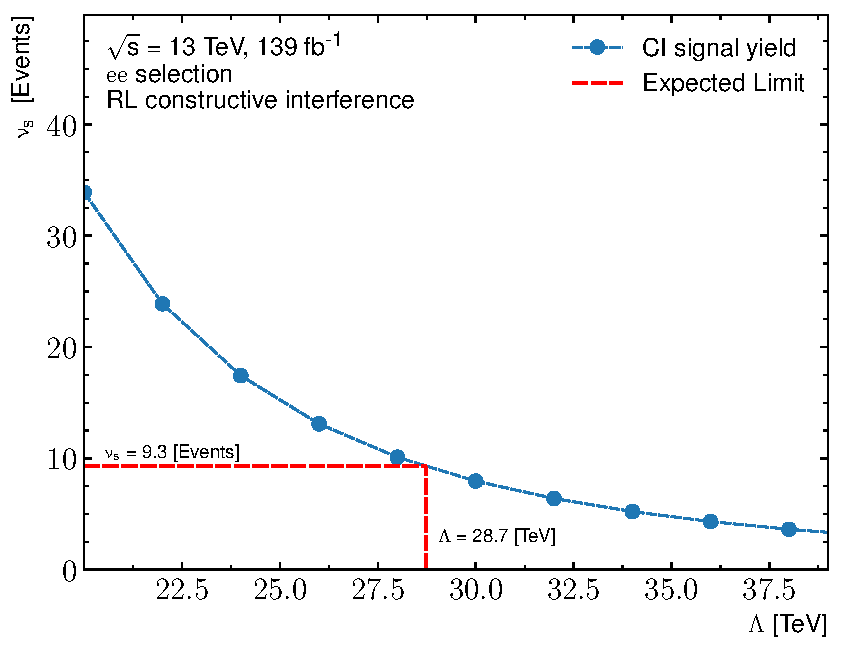
\includegraphics[width=\textwidth]{/Users/Deshan/Documents/PhD/thesis/Thesis/figures/analysis/stats/intersection-ee-const-RL.pdf}
        \label{fig:bkgmodel:interpee3}
    \end{subfigure}
    \begin{subfigure}[b]{0.49\textwidth}
        \centering
        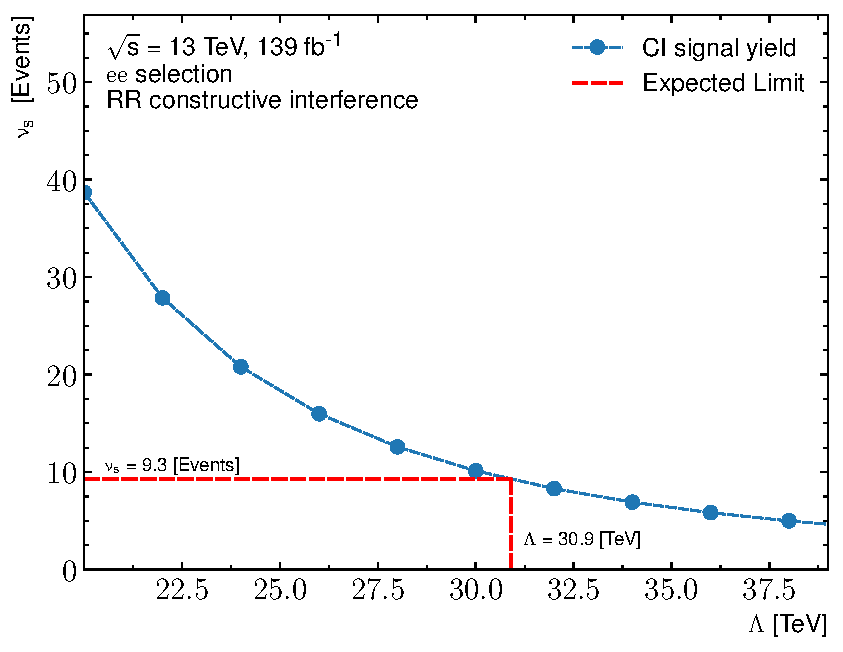
\includegraphics[width=\textwidth]{/Users/Deshan/Documents/PhD/thesis/Thesis/figures/analysis/stats/intersection-ee-const-RR.pdf}
        \label{fig:bkgmodel:interpee4}
    \end{subfigure}
    \caption{Distribution of the expected yield in the signal region corresponding to $\Lambda$ values. The expected limit on the number of signal events is depicted and the mapping to it's $\Lambda$ value. The constructive interference signal regions are shown for the electron channel.}
    \label{fig:stats:interpeeconst}
\end{figure}

\begin{figure}[h!]
    \centering
    \begin{subfigure}[b]{0.49\textwidth}
        \centering
        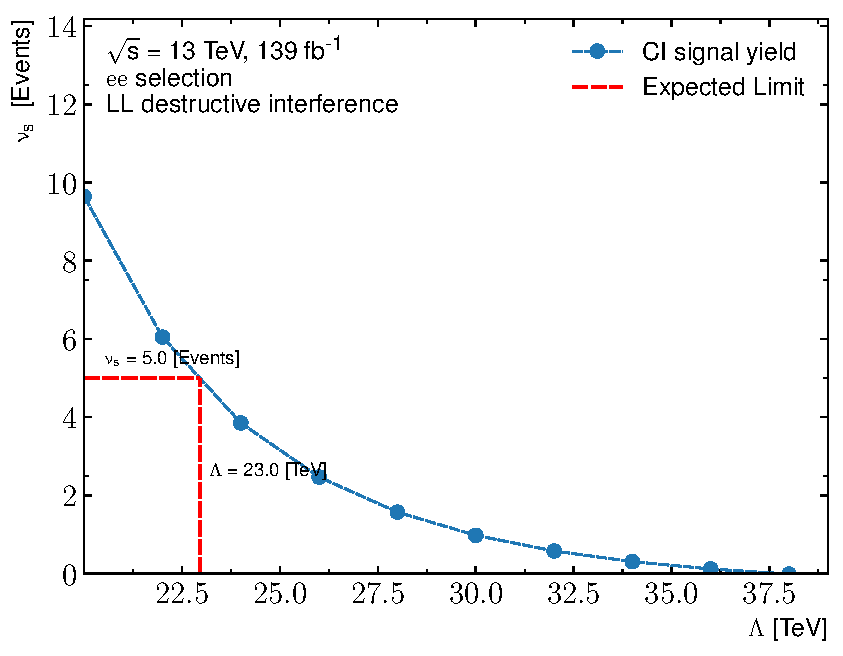
\includegraphics[width=\textwidth]{/Users/Deshan/Documents/PhD/thesis/Thesis/figures/analysis/stats/intersection-ee-dest-LL.pdf}
        \label{fig:bkgmodel:interpee5}
    \end{subfigure}
    \begin{subfigure}[b]{0.49\textwidth}
        \centering
        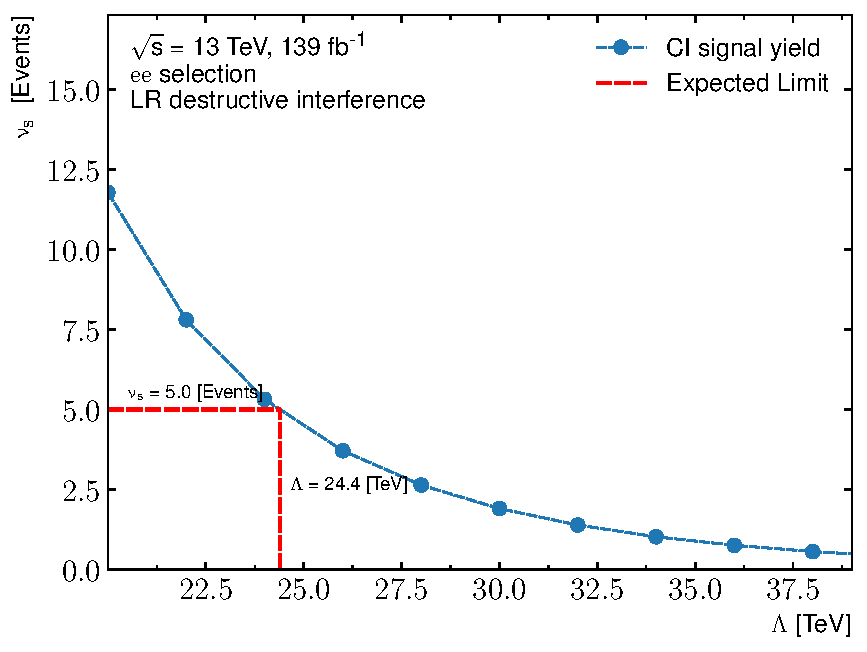
\includegraphics[width=\textwidth]{/Users/Deshan/Documents/PhD/thesis/Thesis/figures/analysis/stats/intersection-ee-dest-LR.pdf}
        \label{fig:bkgmodel:interpee6}
    \end{subfigure}
    \begin{subfigure}[b]{0.49\textwidth}
        \centering
        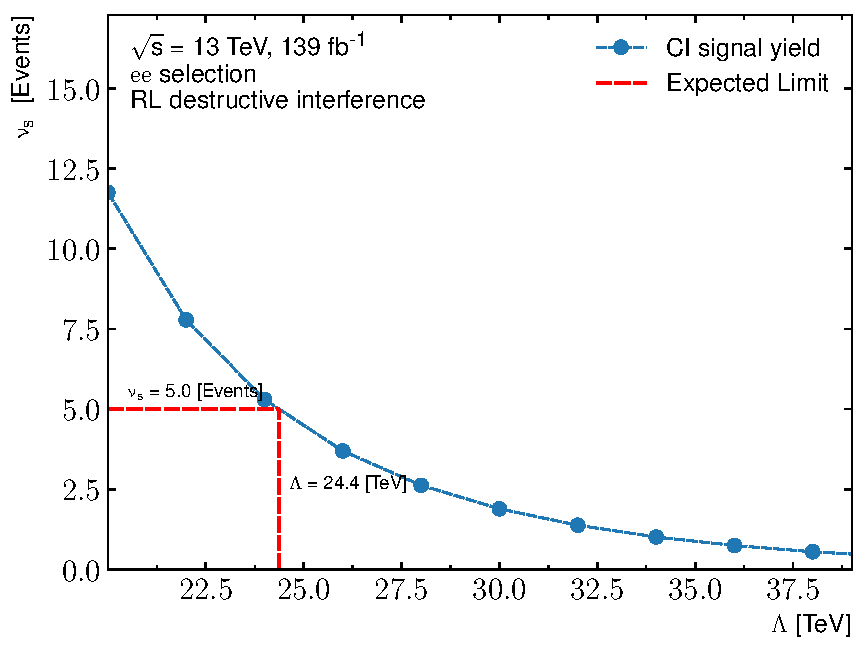
\includegraphics[width=\textwidth]{/Users/Deshan/Documents/PhD/thesis/Thesis/figures/analysis/stats/intersection-ee-dest-RL.pdf}
        \label{fig:bkgmodel:interpee7}
    \end{subfigure}
    \begin{subfigure}[b]{0.49\textwidth}
        \centering
        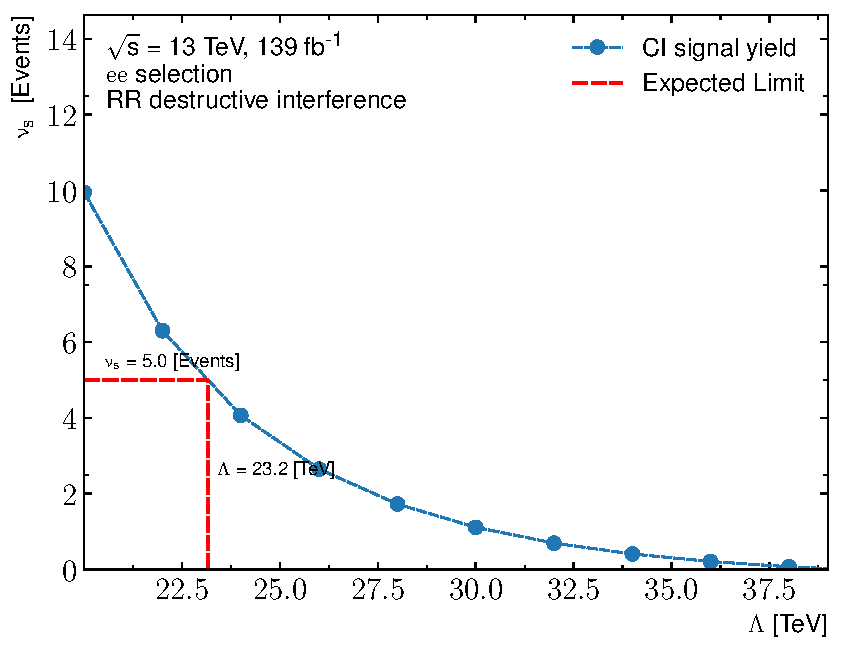
\includegraphics[width=\textwidth]{/Users/Deshan/Documents/PhD/thesis/Thesis/figures/analysis/stats/intersection-ee-dest-RR.pdf}
        \label{fig:bkgmodel:interpee8}
    \end{subfigure}
    \caption{Distribution of the expected yield in the signal region corresponding to $\Lambda$ values. The expected limit on the number of signal events is depicted and the mapping to it's $\Lambda$ value. The destructive interference signal regions are shown for the electron channel.}
    \label{fig:stats:interpeedest}
\end{figure}

\begin{figure}[h!]
    \centering
    \begin{subfigure}[b]{0.49\textwidth}
        \centering
        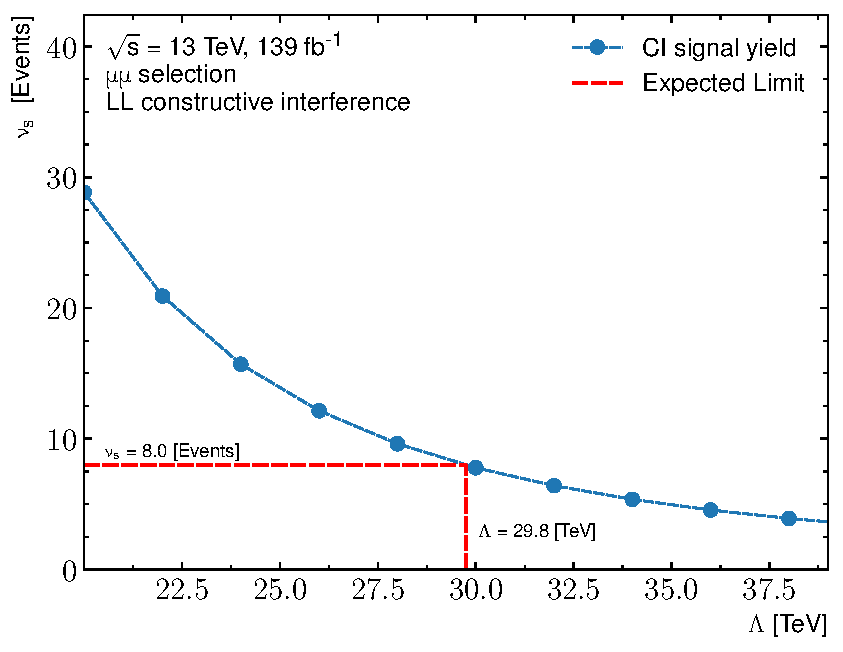
\includegraphics[width=\textwidth]{/Users/Deshan/Documents/PhD/thesis/Thesis/figures/analysis/stats/intersection-mm-const-LL.pdf}
        \label{fig:bkgmodel:interpmm1}
    \end{subfigure}
    \begin{subfigure}[b]{0.49\textwidth}
        \centering
        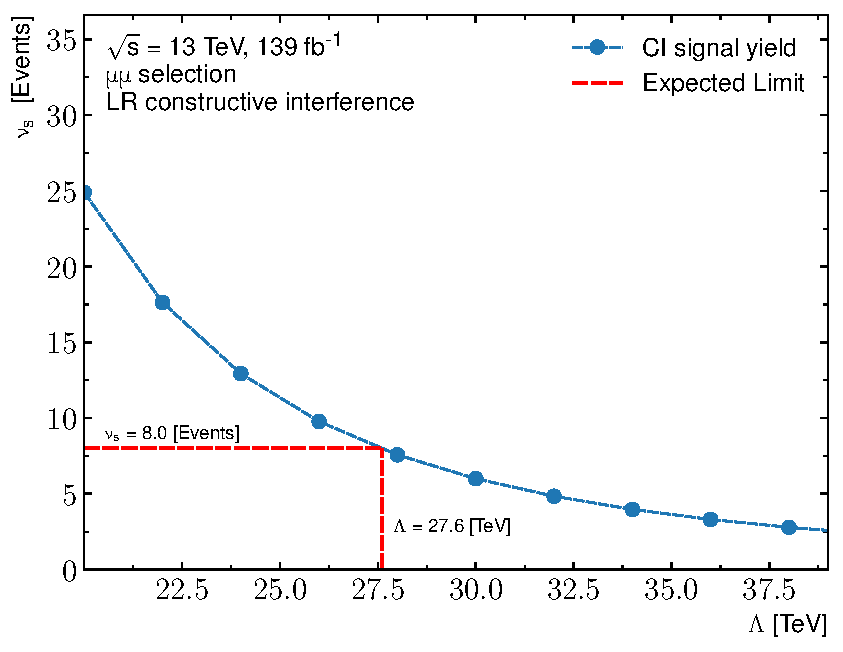
\includegraphics[width=\textwidth]{/Users/Deshan/Documents/PhD/thesis/Thesis/figures/analysis/stats/intersection-mm-const-LR.pdf}
        \label{fig:bkgmodel:interpmm2}
    \end{subfigure}
    \begin{subfigure}[b]{0.49\textwidth}
        \centering
        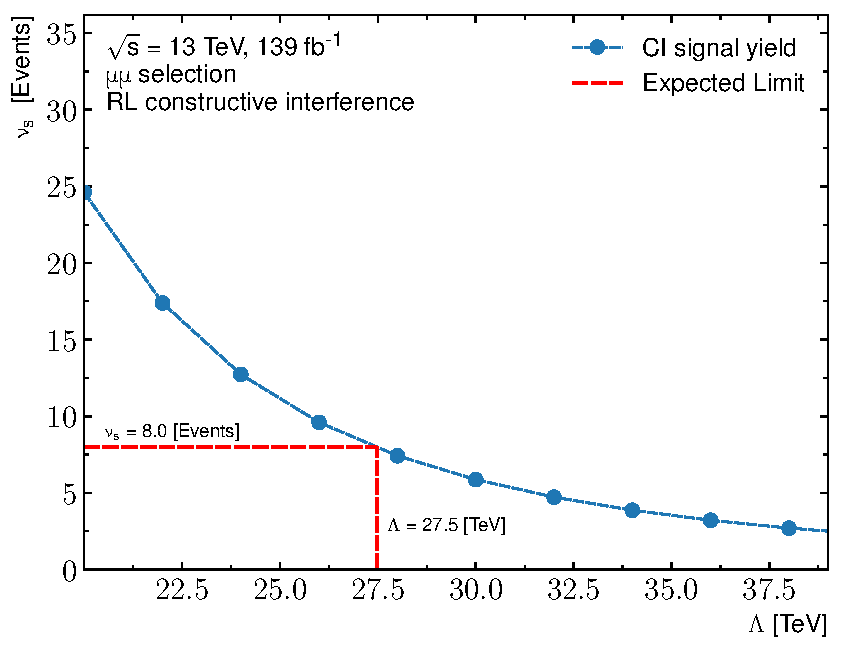
\includegraphics[width=\textwidth]{/Users/Deshan/Documents/PhD/thesis/Thesis/figures/analysis/stats/intersection-mm-const-RL.pdf}
        \label{fig:bkgmodel:interpmm3}
    \end{subfigure}
    \begin{subfigure}[b]{0.49\textwidth}
        \centering
        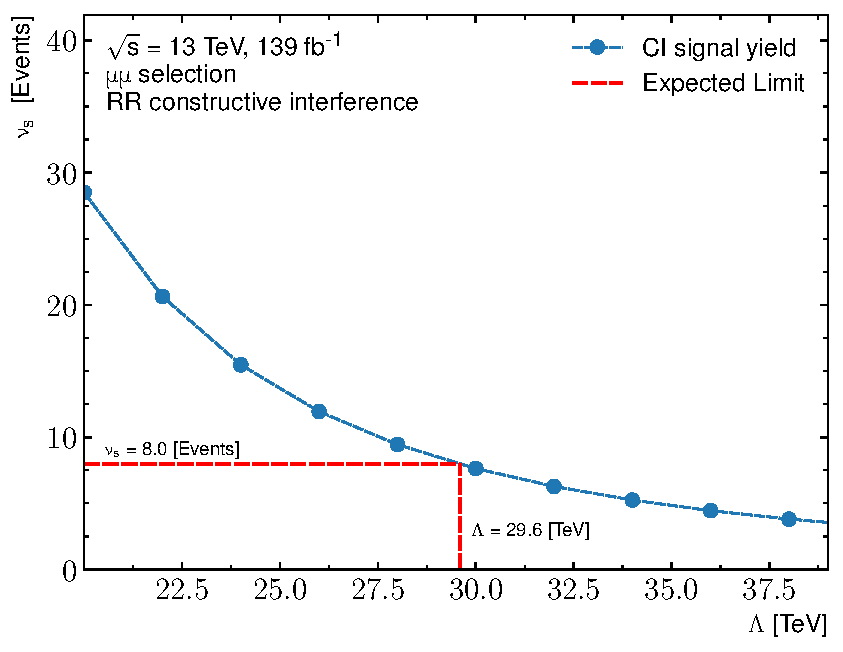
\includegraphics[width=\textwidth]{/Users/Deshan/Documents/PhD/thesis/Thesis/figures/analysis/stats/intersection-mm-const-RR.pdf}
        \label{fig:bkgmodel:interpmm4}
    \end{subfigure}
    \caption{Distribution of the expected yield in the signal region corresponding to $\Lambda$ values. The expected limit on the number of signal events is depicted and the mapping to it's $\Lambda$ value. The constructive interference signal regions are shown for the muon channel.}
    \label{fig:stats:interpmmconst}
\end{figure}

\begin{figure}[h!]
    \centering
    \begin{subfigure}[b]{0.49\textwidth}
        \centering
        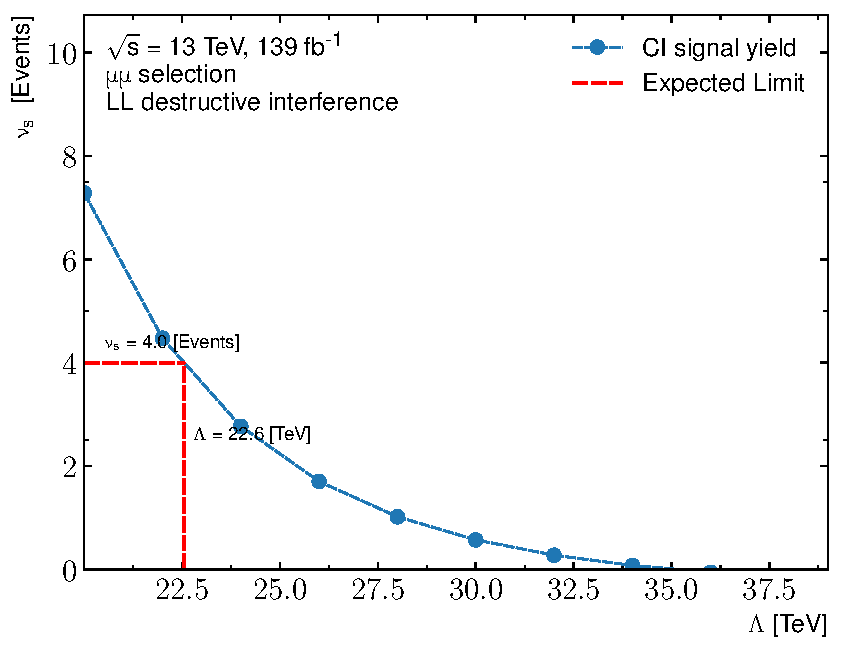
\includegraphics[width=\textwidth]{/Users/Deshan/Documents/PhD/thesis/Thesis/figures/analysis/stats/intersection-mm-dest-LL.pdf}
        \label{fig:bkgmodel:interpmm5}
    \end{subfigure}
    \begin{subfigure}[b]{0.49\textwidth}
        \centering
        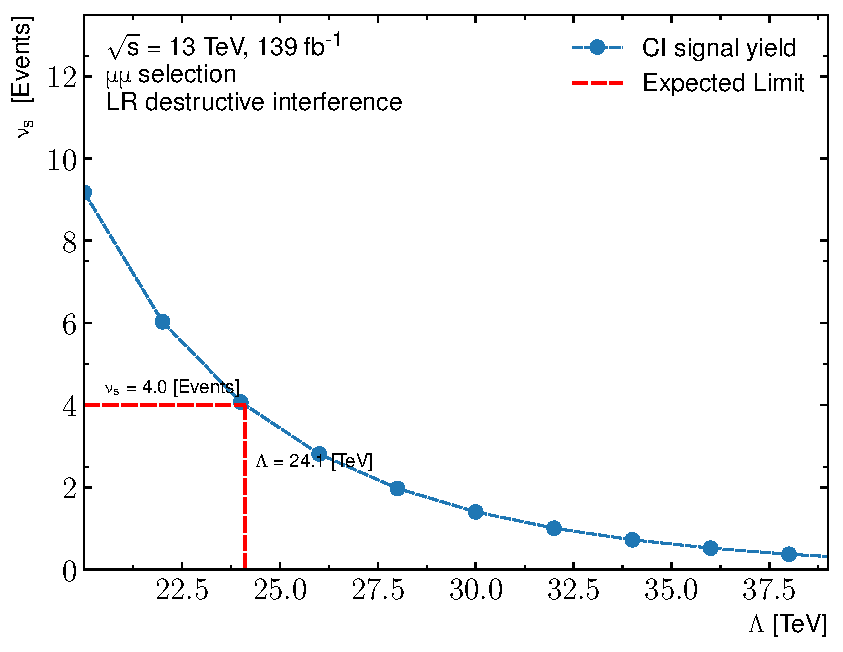
\includegraphics[width=\textwidth]{/Users/Deshan/Documents/PhD/thesis/Thesis/figures/analysis/stats/intersection-mm-dest-LR.pdf}
        \label{fig:bkgmodel:interpmm6}
    \end{subfigure}
    \begin{subfigure}[b]{0.49\textwidth}
        \centering
        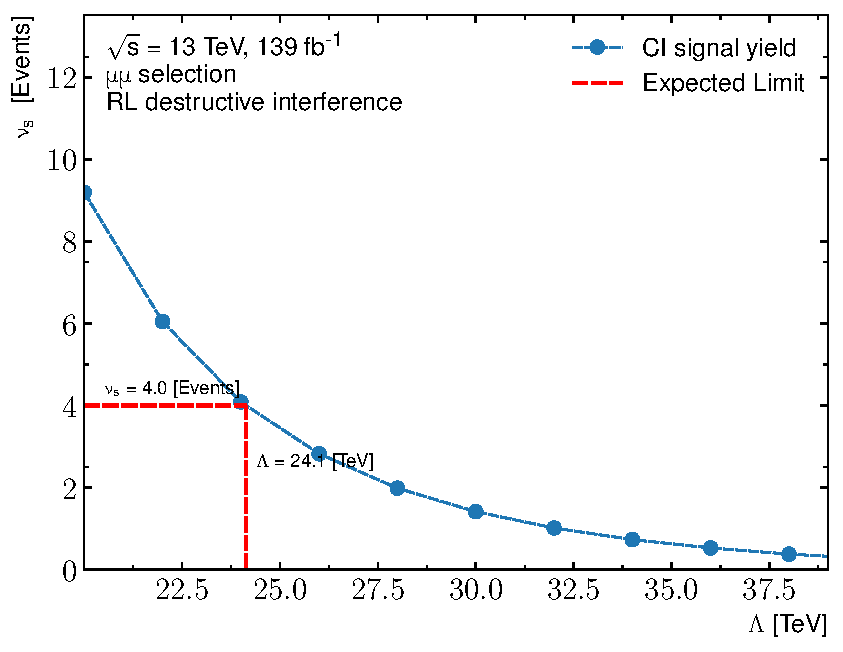
\includegraphics[width=\textwidth]{/Users/Deshan/Documents/PhD/thesis/Thesis/figures/analysis/stats/intersection-mm-dest-RL.pdf}
        \label{fig:bkgmodel:interpmm7}
    \end{subfigure}
    \begin{subfigure}[b]{0.49\textwidth}
        \centering
        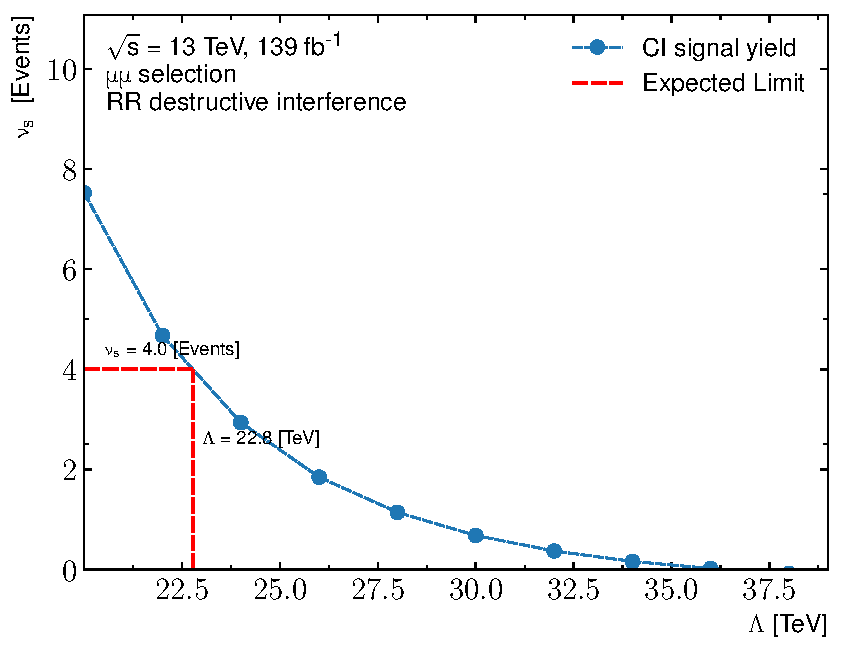
\includegraphics[width=\textwidth]{/Users/Deshan/Documents/PhD/thesis/Thesis/figures/analysis/stats/intersection-mm-dest-RR.pdf}
        \label{fig:bkgmodel:interpmm8}
    \end{subfigure}
    \caption{Distribution of the expected yield in the signal region corresponding to $\Lambda$ values. The expected limit on the number of signal events is depicted and the mapping to it's $\Lambda$ value. The destructive interference signal regions are shown for the muon channel.}
    \label{fig:stats:interpmmdest}
\end{figure}

\begin{table}[htp]
    \begin{center}  
{\begin{tabular}{r c c c c c c c c c c c}\toprule
    & & & \multicolumn{4}{c}{Expected limit [TeV]} \\
    Int. & Channel & POI & LL & LR & RL & RR \\
    \midrule
    \multirow{3}{*}[-1em]{\begin{sideways}Constructive\end{sideways}} & \multirow{2}{*}{$\ee$} & $\Lambda$ & 31.1 & 28.9 & 28.7 & 30.9 \\
    & & $\nu_s$ & 31.1 & 28.8 & 28.7 & 30.9 \\
    \cmidrule{2-7}
     & \multirow{2}{*}{$\mumu$} & $\Lambda$ & 29.8 & 27.6 & 27.5 & 29.6 \\
    & & $\nu_s$ & 29.8 & 27.6 & 27.5 & 29.6 \\
    \midrule
    \multirow{3}{*}[-1em]{\begin{sideways}Destructive\end{sideways}} & \multirow{2}{*}{$\ee$} & $\Lambda$ & 23.0 & 24.4 & 24.4 & 23.2 \\
    & & $\nu_s$ & 23.0 & 24.4 & 24.4 & 23.2 \\
    \cmidrule{2-7}
     & \multirow{2}{*}{$\mumu$} & $\Lambda$ & 22.6 & 24.0 & 24.2 & 22.8 \\
    & & $\nu_s$ & 22.6 & 24.1 & 24.1 & 22.8 \\
\bottomrule\end{tabular}}
\caption{Comparison of expected limits from reinterpreting the results in terms of $\Lambda$ from limits on the number of signal events ($\nu_s$) and limits set directly on $\Lambda$ as the parameter of interest. The limits are shown for the various CI chiral and interference models in the electron and muon channels.}  
\label{tab:limits_comparePOI}
\end{center}
\end{table}

\clearpage
